\chapter{Electrically generated eddies at an eight-fold stagnation point
within a nanopore}\label{chpt:eddies}
\section{Introduction}
Streamline patterns reveal the topology of a flow field:
we sketch streamlines, eddies and stagnation points
in order to develop our understanding of flows
\cite{moffatt1964,jeffrey1980}.
Stagnation points away from solid walls usually occur at the intersection of
two streamlines, which divide the fluid into four separate regions.
Such stagnation points can be generated in many ways, e.g. by
a four-roll mill \cite{taylor1934} or by opposed fluid jets
in a cross-slot device \cite{scrivener1979,cachile2012}.
More complicated stagnation points are harder to generate.
Berry and Mackley \cite{berry1977} built  a six-roll mill and investigated
the flow field. When exact symmetry was achieved,
six eddies met at a central point, and the various ways in which
symmetry could be broken were described by Berry and Mackley
in terms of catastrophe theory. Here we report an electrically
generated flow
field in which four streamlines cross at a point and divide the flow into eight
regions.


\begin{figure}[ht]
\begin{center}
\includegraphics[width=0.8\textwidth,clip=true]{eddies/eddy_fig1b.eps}
\end{center}
\caption{The (infinite)
dielectric plate of thickness $h$, pierced by a hole of radius $a$
and surrounded by
an electrolyte solution. 
The axisymmetric geometry represents a nanopore in a membrane.
An electrical current is driven through the hole by a potential difference
$\Delta\phi$ between the two sides, at infinity.}
\label{fig:hole}
\end{figure}


The axisymmetric flow geometry is shown in figure \ref{fig:hole}.
A cylindrical
hole of radius $a$ passes through an uncharged thin dielectric
plate of thickness $h$:
the hole represents a nanopore in a membrane, and we are interested in the
induced charge electroosmotic
flow generated by an electric potential difference applied 
between the two sides of the membrane \cite{Mao2013,mao2014,sherwood2014}.
We set up cylindrical polar coordinates, with $z$ axis along the axis of
symmetry and with the plane surfaces of the membrane at $r>a$,  $z=\pm h/2$.

In Section \ref{sec:imposed_electric} we consider the electric field passing through a circular hole in
a membrane of zero thickness. We then (Section \ref{sec:conformal_map})
show how the field is modified at
the edge of the hole when the membrane thickness $h$ is small but non-zero.
In Section \ref{sec:corner_charge}
we review the fluid jets that are created by the electrical
forces on 
%%%
the
%%%
fluid near the
corners of the membrane, and then in Section \ref{numerical_comp} we present 
numerical computations that show how the geometry of
eddies created by these jets depends on the geometry of the hole in
the membrane. As the ratio $h/a$ increases, three
stagnation points merge to form
a stagnation point at which four streamlines cross. The
stagnation points separate again
as $h/a$ increases further.

\section{The imposed electric field\label{sec:imposed_electric}}

The pore
and the two regions on either side of the membrane are occupied by
an incompressible, electrically conducting
Newtonian electrolyte solution
with viscosity $\mu$ and electrical permittivty
$\epsilon_f$. The membrane is non-conducting, with permittivity $\epsilon_s$.
The electrical potential $\phi$ is continuous at the boundary
between the solid membrane and the fluid.
The surface charge density
on the membrane is zero, so that
$\epsilon\mathbf n\cdot\nabla\phi$ is continuous,
where $\mathbf n$ is the unit normal to the membrane
and the permittivity $\epsilon$ takes values $\epsilon_s$ and
$\epsilon_f$ on the two sides of the boundary. If (as is usually
the case) $\epsilon_s\ll\epsilon_f$, then to a first approximation
we set $\epsilon_s=0$, and
$\mathbf n\cdot\nabla\phi=0$ in the fluid adjacent to the membrane.

We assume that the electrolyte solution
contains $N$ ionic species,
with valence $z_i$ and number density $n^i$.
Far from any charged surfaces, the ionic
number densities are $n^i=n^i_\infty$, with $\sum_i z_in_\infty^i=0$
to ensure electrical neutrality of the bulk electrolyte.
The electrical potential satisfies the Poisson equation
\begin{equation}
\nabla^2\phi=-\rho/\epsilon_f=-\sum_{i=1}^Nez_in^i/\epsilon_f,
\label{poisson}
\end{equation}
where $\rho$ is the charge density.

Ions are convected with the fluid velocity $\mathbf{u}$, and move relative
to the fluid under the influence of electric fields and thermal diffusion.
The
conservation equation for the number density
$n^i$ of the $i$th ionic species, in steady state, is
therefore
\begin{equation}
\nabla\cdot\left\lbrack n^i\mathbf{u} -\omega_i(kT\nabla
n^i + ez_in^i\nabla\phi) \right\rbrack=0,
\label{ion_conservation}
\end{equation}
where $\omega_i$ is the mobility of the $i$th species of ion, $kT$ is
the Boltzmann temperature, and $e$ is the elementary charge.
In the absence of any reactions at the surface of the membrane,
the flux of ions normal to the membrane is zero at the membrane surface. 

If $\epsilon_s=0$, there is a steady
solution of the ion conservation equation (\ref{ion_conservation})
in which the fluid is at rest ($\mathbf u=0$), the ionic
number densities are unperturbed ($n^i=n_\infty^i$),
and the electrical potential $\phi=\phi_0$ within the electrolyte
is given by the solution of the Laplace equation
\begin{subeqnarray}
\nabla^2\phi_0&=&0,
\\
\mathbf{n}\cdot\nabla\phi_0&=&0\hskip 20pt\hbox{on the membrane surface,}
\slabel{neumann_bc}
\\
\phi&\rightarrow&\pm\Delta\phi/2,\quad
\hbox{as $\mathbf{r}\rightarrow\infty$ in $z\gtrless 0$.}
\label{ohmic_chi_defn}
\end{subeqnarray}
This represents Ohmic
conduction through an electrolyte with uniform electrical conductivity.
The solution $\phi_0=\Phi_0$
of the Laplace equation (\ref{ohmic_chi_defn})
when $h=0$ is given by Morse and Feshbach \cite{M&F} (p. 1292)
in terms of
oblate spherical coordinates $(\xi,\eta)$
where $-\infty < \xi <\infty$, $0 \leq \eta \leq \pi/2$ such that
\begin{equation}
z=a\sinh\xi\cos\eta\quad,\quad r=a\cosh\xi\sin\eta,
\end{equation}
and is
\begin{subeqnarray}
\phi_0=\Phi_0(r,z)& =& \frac{\Delta \phi}{2} \left[ 1- \frac{2}{\pi}
\tan^{-1}\left( \frac{1}{\sinh \xi} \right) \right],\quad z>0,\quad h=0,
\\
&=&-\Phi_0(r,-z),\quad z<0.
\label{eq:chi_eddies}
\end{subeqnarray}
On the surface $z=0_+$ of the membrane
\begin{equation}
\Phi_0(r,0_+) = \frac{\Delta \phi}{2} \left[ 1- \frac{2}{\pi}
\tan^{-1}\left( \frac{a}{(r^2-a^2)^{1/2}} \right) \right],
\quad r>a,
\label{eq:chi_eddies_z0}
\end{equation}
and for $r=a(1+\delta)$, with $\delta\ll 1$,
\begin{equation}
\Phi_0(r,0_+)\approx \frac{\Delta\phi}{\pi}(2\delta)^{1/2},
\label{eq:chi_eddies_z0_delta}
\end{equation}
with $\Phi_0(r,0_-)=-\Phi_0(r,0_+)$. The electric field in the plane
of the hole is
\begin{equation}
\mathbf{E}=-
\frac{\Delta\phi\ \hat{\mathbf{z}}}{\pi a\left(1-r^2/a^2\right)^{1/2}},
\quad r<a,
\label{Ez_hole}
\end{equation}
and if the conductivity of the electrolyte is $\Sigma$, the total
current through the hole is $2 a\Sigma\Delta\phi$.
However, real membranes have a non-zero thickness $h>0$.
We shall show in Section \ref{sec:conformal_map} that when $0<h\ll a$,
the potential
$\phi_0$
differs from the potential $\Phi_0$ for $h=0$ by an amount $O((h/a)^{1/2})$.
We neglect this perturbation for the moment, and assume
$\phi_0(r,h/2)\approx\Phi_0(r,0_+)$.
The leading order potential $\phi_0$
leads to an electric field of strength 
\begin{equation}
\hat{\mathbf{z}}\cdot\nabla\phi=\frac{2\phi_0(r,h/2)}{h}\approx \frac{2\Phi_0(r,0_+)}{h}
\label{internal_field}
\end{equation}
within the membrane.


If $\epsilon_s=0$ (as assumed so far), the electric field
(\ref{internal_field}) within the
membrane and the electric field (\ref{neumann_bc})
outside the membrane satisfy the requirement
that $\epsilon\mathbf n\cdot\nabla\phi$ 
should be continuous at the boundary.
However, in the real world, $\epsilon_s$ is at least as large
as the permittivity of free space, $\epsilon_0$, so that
$\epsilon_s\ge \epsilon_0>0$, and
the normal electric field outside the membrane
must be perturbed at $O(\epsilon_s\Delta\phi/(\epsilon_f h))$
in order to ensure continuity of $\epsilon\mathbf n\cdot\nabla\phi$.
Ions move towards (or away from)
the membrane under the influence
of this perturbation until equilibrium, with zero flux of ions
into the membrane, is achieved.
In order to determine this perturbation to the field, we assume that
\begin{equation}
\gamma=\frac{\epsilon_s}{\epsilon_f}\ll 1
\end{equation}
and use $\gamma$ as the basis
for a perturbation expansion:
\begin{subeqnarray}
\phi &=& \phi_0 + \gamma\phi_1 +\cdots,\\
n^i &=& n_0^i + \gamma n_1^i +\cdots,\\
{\mathbf{u}} &=&\hskip 28pt  \gamma{\mathbf{u}}_1 + \cdots,
\end{subeqnarray}
where the subscript 0 refers to the uniform ion density $n_0^i=n_\infty^i$
and to the potential (\ref{ohmic_chi_defn}) for $\epsilon_s=0$. The
$O(\gamma)$ terms in the
steady-state ion conservation equation give
\begin{equation}
{\mathbf{u}}_1\cdot\nabla n_0^i = \omega_i\nabla\cdot\left\lbrack
ez_in_0^i\nabla\phi_1 + ez_in_1^i\nabla\phi_0 
+kT\nabla n_1^i \right\rbrack,
\label{convdiff_eddies}
\end{equation}
Since
$n_0^i$ is uniform, the left-hand side of (\ref{convdiff_eddies}) is zero.

On the surface of the membrane, (except close to the edge of the hole),
the potential $\phi_0$
varies on a length scale $r>a$, whereas we expect the perturbation potential
$\phi_1$ to vary on the Debye length scale
\begin{equation}
\kappa^{-1}=\left(
\frac{\epsilon_f kT}{\sum_{i=1}^N e^2 z_i^2n_\infty^i}\right)^{1/2}.
\end{equation}
Hence, if $r-a\gg\kappa^{-1}$ so that
we are much further than a Debye length away from the edge of the hole,
we may
neglect the second term on the
right-hand side of (\ref{convdiff_eddies}), which reduces to
\begin{equation}
\nabla\cdot\left\lbrack
ez_in_0^i\nabla\phi_1  +kT\nabla
n_1^i \right\rbrack=0,
\label{convdiff_eddies2}
\end{equation}
The perturbed ionic number densities are therefore given by a Boltzmann
distribution
\begin{equation}
n_1^i=n_\infty^i\text{e}^{-ez_i\phi_1/kT}
\end{equation}
and $\phi_1$ satisfies the Poisson equation
\begin{equation}
\nabla^2\phi_1=-\frac{\rho_1}{\epsilon_f}
=-\frac{e}{\epsilon_f}\sum_{i=1}^N
z_in_1^i
=-\frac{e}{\epsilon_f}\sum_{i=1}^Nz_in_\infty^i\text{e}^{-ez_i\phi_1/kT}.
\label{poisson1}
\end{equation}
The perturbation potential $\phi_1$ varies in the $z$ direction over
the Debye length scale $\kappa^{-1}$, and we neglect its slow variation
with $r$. 
We assume that
$\gamma e\phi_1/(kT)$ is small, and linearize the
Poisson-Boltzmann equation (\ref{poisson1}), which becomes
\begin{equation}
\frac{\text{d}^2\phi_1}{\text{d}z^2}=-\kappa^2\phi_1.
\label{linear_PB_eqn}
\end{equation}
The solution of (\ref{linear_PB_eqn})
that ensures that the potential $\phi=\phi_0+\gamma\phi_1$
satisfies the jump boundary condition $[\epsilon\mathbf n\cdot\nabla\phi]=0$
at the surface of the membrane is
\begin{subeqnarray}
\phi&=&\phi_0
-\frac{2\Phi_0(r,0_+)\epsilon_s}{h\kappa\epsilon_f+2\epsilon_s}
\exp[-\kappa(z-h/2)],\hskip 20pt z>h/2,
\\
\phi&=&\phi_0
+\frac{2\Phi_0(r,0_+)\epsilon_s}{h\kappa\epsilon_f+2\epsilon_s}
\exp[\kappa(z+h/2)],\hskip 20pt z<-h/2,
\label{ICEO_external_pot_perturbation}
\end{subeqnarray}
with
\begin{equation}
\phi=\frac{2\Phi_0(r,0_+)\kappa\epsilon_f z}{h\kappa\epsilon_f+2\epsilon_s}
,\hskip 20pt |z|<h/2,
\label{ICEO_internal_pot_perturbation}
\end{equation}
inside the solid membrane. We see from (\ref{ICEO_external_pot_perturbation})
that the perturbation $\gamma\phi_1$ is only small compared to $\phi_0$
if $\gamma/(h\kappa)\ll 1$. 
We also note that
(\ref{ICEO_external_pot_perturbation})
does not represent the first terms of a systematic expansion,
and is incorrect at $O((\gamma/h\kappa)^2)$.
However, we prefer to leave the expansion in
the form (\ref{ICEO_external_pot_perturbation}) since it shows explicitly
how the expansion fails in the limit $h\rightarrow 0$.
In particular, far from the hole we recover the
uniform charge cloud that would be induced in the absence of any hole.
A detailed analysis
of induced charge electroosmotic flow around
an uncharged dielectric
sphere (or cylinder)
of radius $a$ in the limit $a\kappa\gg 1$ has been provided by Schnitzer \&
Yariv \cite{schnitzer2014strong}.

The perturbation potential (\ref{ICEO_external_pot_perturbation})
outside the membrane can be described in terms of an
effective induced zeta potential
\begin{equation}
\zeta_i=-\frac{2\epsilon_s\Phi_0(r,0_+)}{h\kappa\epsilon_f+2\epsilon_s}.
\label{zeta_induced}
\end{equation}

The tangential electric field $-\partial\phi/\partial r$ acts on
the charge cloud adjacent to the membrane and causes a tangential
velocity. Immediately outside the double layer
(assuming $r\gg a+\kappa^{-1}$, so that
flow can be assumed to be locally one-dimensional), the leading-order 
radial fluid
velocity outside the charge cloud is given by the Smoluchowski slip velocity
\begin{equation}
u=\frac{\partial\phi}{\partial r}\frac{\epsilon_f\zeta_i}{\mu},
\end{equation}
and using the expansion (\ref{eq:chi_eddies_z0_delta}) at $r=a(1+\delta)$,
together with
(\ref{zeta_induced}), we obtain, in the limit $\epsilon_s\ll h\kappa\epsilon_f$,
\begin{equation}
u=-\frac{2\epsilon_\text{s}}{ah\kappa\mu}\left(\frac{\Delta\phi}{\pi}\right)^2
,\hskip 20pt z=0_+.
\label{u_thin_plane}
\end{equation}
The radial velocity created by the induced charge is towards the hole
on both sides of the membrane.

This solution (\ref{ICEO_external_pot_perturbation}),
(\ref{ICEO_internal_pot_perturbation}), (\ref{u_thin_plane})
is clearly inappropriate within a distance $O(\kappa^{-1})$ of the
edge of the hole, where the electric field can
no longer be assumed to vary slowly with $r$.
In the next section, we find a local solution
to the Laplace equation in the neighbourhood of the edge,
for the case $\epsilon_s=0$ for which the electric field
satisfies a Neumann boundary condition (\ref{neumann_bc})
at the surface of the membrane.

\section{Membrane of uniform thickness: a conformal mapping solution
\label{sec:conformal_map}}

\begin{figure}[ht]
\begin{center}
\includegraphics[width=0.9\textwidth,clip=true]{eddies/eddy_fig2a.eps}
\caption{(a) The $Z$ plane, with origin at C. D is at $Z=1$ and B at $Z=-1$.
(b) The $w$ plane, with origin at D$'$. C$'$ is at $w=-\text{i}H\pi/2$
and B$'$ is at $w=-\text{i}H\pi$. The $w$ plane represents the edge of the hole
in the membrane. \label{fig:z_plane}}
\end{center}
\end{figure}

We now study in detail the electric field
at the edge of the membrane of thickness $h>0$ near $r=a$,
for the case $\epsilon_s=0$. Sufficiently close
to the edge (Figure \ref{fig:z_plane}(b)) we neglect the azimuthal curvature,
and seek a local solution of the two-dimensional Laplace equation.
In the limit $h\ll a$, the outer limit of the
local solution can then be matched
to the inner limit
(\ref{eq:chi_eddies_z0_delta}) of the outer solution
for a membrane of zero thickness.

We map the upper half
of the $Z$-plane $Z=X+\text{i}Y$ (Figure \ref{fig:z_plane}(a)) onto the region outside a
rectangular edge in the $w$ plane $w=u+\text{i}v$ (Figure \ref{fig:z_plane}(b))
by means of the conformal mapping \cite{driscoll2002}
\begin{equation}
w=H\left\lbrack Z(Z^2-1)^{1/2}-\cosh^{-1}(Z)\right\rbrack,
\label{conformal_mapping}
\end{equation}
where the constant $H$ will be determined later, and
the branch of the square root is chosen such that
\begin{equation}
w=H\left\lbrack X(X^2-1)^{1/2}-\ln(X+(X^2-1)^{1/2})\right\rbrack,
\hskip 10pt Z=X\ge 1,
\end{equation}
along the real axis.
The rectangular edge (Figure \ref{fig:z_plane}(b)) represents the right-hand edge of the 
hole in the membrane (Figure \ref{fig:hole}), seen on a scale at which the membrane thickness
can be observed, and
the constant $H$ in (\ref{conformal_mapping}) will eventually be chosen
to ensure that the membrane has thickness $h$.

If $Z=X\gg 1$ (E on Figure \ref{fig:z_plane}(a)),
\begin{equation}
w\sim HX^2.
\end{equation}
If $Z=1+\varepsilon$, with $|\varepsilon|\ll 1$
 (near D on Figure \ref{fig:z_plane}(a)), then 
\begin{equation}
w=H\left(\frac{4\sqrt 2}{3}\right)\varepsilon^{3/2}.
\label{near_D}
\end{equation}
so that if $Z=1-\varepsilon_R$, with $0<\varepsilon_R\ll 1$
real,
\begin{equation}
w=-H\left(\frac{4\sqrt 2}{3}\right)\varepsilon_R^{3/2}\text{i},
\end{equation}
and if $Z=\varepsilon$ with
$|\varepsilon|\ll 1$ (near C on Figure \ref{fig:z_plane}(a)),
\begin{equation}
w
=-\text{i}H\left\lbrack \frac{\pi}{2}-2\varepsilon\right\rbrack.
\end{equation}
Finally, since $\cosh^{-1}(-Z)=\pi \text{i}-\cosh^{-1}Z$,
we note that when $Z=-1$
(at B),
\begin{equation}
w=-H\cosh^{-1}Z=-\text{i}H\pi.
\label{at_B}
\end{equation}
In order to map the upper half $Z$ plane into the space outside a
semi-infinite rectangular slab of
thickness $|\text{D}'\text{B}'|=h$, we see from (\ref{near_D}) and (\ref{at_B})
that we should choose $H=h/\pi$.

We now consider the (harmonic) function
\begin{equation}
\phi=CH^{1/2}\Re(Z)=CH^{1/2}X.
\end{equation}
This satisfies the Neumann boundary condition (\ref{neumann_bc})
on the boundary ABCDE
in the $Z$ plane, and after transformation to the $w$ plane leads to a
solution \cite{M&F} of the Laplace equation
that satisfies the Neumann boundary
condition on the transformed boundary
A$'$B$'$C$'$D$'$E$'$, i.e. on the
boundary of the membrane near the
edge of the hole.
In the far field of the $w$ plane
\begin{equation}
\phi=C\Re(w^{1/2}),
\end{equation}
which matches with the inner expansion of the outer solution
(\ref{eq:chi_eddies_z0_delta}) for the electric potential
at the edge of the hole in a membrane
of zero thickness if
\begin{equation}
C=\left(\frac{2}{a}\right)^{1/2}\frac{\Delta\phi}{\pi}.
\end{equation}
Close to the corner D$'$ of the slab, at $w=s\,\text{e}^{\text{i}\theta}$
with $s\ll 1$,
\begin{equation}
\phi=CH^{1/2}\left\lbrace 1+\left(\frac{3s}{4H\sqrt2}\right)^{2/3}
\cos\left(\frac{2\theta}{3}\right)
\right\rbrace.
\label{local_soln_expanded}
\end{equation}
Thus the electrical potential at the corner D$'$ is
$CH^{1/2}=\Delta\phi (2h/a)^{1/2} \pi^{-3/2}$, together with an eigensolution
proportional to $s^\lambda$,
with $\lambda=2/3$, and
the potential difference between the two corners $\text D'$ and $\text B'$
(Figure \ref{fig:z_plane}) is
\begin{equation}
\Delta\phi_c=\Delta\phi\left(\frac{2}{\pi}\right)^{3/2}\left(\frac{h}{a}\right)^{1/2}.
\label{delta_phi_c}
\end{equation}

In the next section we compare the magnitude of the electroosmotic flow
generated at the corner by the potential (\ref{local_soln_expanded})
with the magnitude of the flow (\ref{u_thin_plane}) generated along the
surface of the membrane away from corners at the edge of the hole.

\section{Induced charge at a corner \label{sec:corner_charge}}


\begin{figure}[ht]
\begin{center}
\includegraphics[width=0.8\textwidth,clip=true]{eddies/eddy_fig3b.eps}

\end{center}

\caption{A dielectric wedge, of angle $2\alpha$, with local
cylindrical coordinates $(s,\theta)$.
\label{fig:corner}}
\end{figure}

The theory of electro-osmotic flow
at a dielectric corner is discussed by Thamida and Chang \cite{Thamida2002} and  Yossifon {\it et al.}
\cite{yossifon2006}.
We consider a plane 2-dimensional
wedge of internal angle $2\alpha=2(\pi-\theta_0)$, and adopt
plane polar coordinates $(s,\theta)$, as shown in Figure \ref{fig:corner}.
The solution of the Laplace equation for the potential $\phi$
outside the electrical double layer, antisymmetric in $\theta$
outside the wedge, has the form
\begin{equation}
\phi=As^\lambda\sin\lambda\theta.
\label{eigensolution}
\end{equation}
Zero flux of ions into the solid wedge requires
\begin{equation}
\mathbf{n}.\nabla\phi=\frac{1}{s}\frac{\partial\phi}{\partial\theta}
=A\lambda s^{\lambda-1}\cos\lambda\theta=0,\hskip 10pt
\theta=\theta_0=\pi-\alpha,
\end{equation}
so that
\begin{equation}
\lambda=\frac{(2n+1)\pi}{2\theta_0},\hskip 20pt n=0,\pm1,\pm2\dots\ .
\end{equation}
If $\theta_0=\pi$, the least singular eigensolution (\ref{eigensolution})
corresponds to $\lambda=1/2$, in agreement with (\ref{eq:chi_eddies_z0_delta}).
If $\alpha=\pi/4$, so
that $\theta_0=3\pi/4$, then $\lambda=2/3$, as found in
(\ref{local_soln_expanded}), and
\begin{equation}
A=\frac{3^{2/3}}{2^{5/3}}CH^{-1/6}
=\frac{3^{2/3}}{2^{7/6}}\frac{\Delta\phi}{\pi a^{1/2}}
\left(\frac{\pi}{h}\right)^{1/6}.
\label{A_corner}
\end{equation}
Within the solid wedge, the potential is
\begin{equation}
\phi=\phi_w=As^\lambda\frac{\sin\lambda\theta_0}{\sin\lambda\alpha}
\sin[\lambda(\pi-\theta)],
\end{equation}
which is antisymmetric about $\theta=\pi$.
As in Section \ref{sec:imposed_electric}, we conclude that there will be an induced
surface charge, corresponding to an induced zeta potential
\begin{subeqnarray}
\zeta_i=-\frac{\epsilon_s}{\kappa\epsilon_f}\frac{\partial\phi_w}{\partial n}
&=&-\frac{\epsilon_s}{\epsilon_f}\frac{As^{\lambda-1}}{\kappa}
\lambda\cot\lambda\alpha\;\sin\lambda\theta_0,\hskip 10pt \theta=\theta_0,
\\
&=&\frac{\epsilon_s}{\epsilon_f}\frac{As^{\lambda-1}}{\kappa}
\lambda\cot\lambda\alpha\;\sin\lambda\theta_0,\hskip 10pt \theta=-\theta_0.
\label{zeta_i_wedge}
\end{subeqnarray}
Note that this potential becomes large
as $s\rightarrow 0$ close to the apex of the wedge, and an analysis based
on linearized Poisson-Boltzmann theory therefore breaks down.
Large induced potentials on the surface of a spherical particle
are discussed by Yariv and Davis \cite{yariv2010}.

The tangential electric field immediately outside the wall is
\begin{subeqnarray}
E_s=-\frac{\partial\Phi_l}{\partial s}
&=&\lambda As^{\lambda-1}\sin\lambda\theta_0,\hskip 10pt \theta=\theta_0,
\\
&=&-\lambda As^{\lambda-1}\sin\lambda\theta_0,\hskip 10pt \theta=-\theta_0,
\end{subeqnarray}
and, as discussed in Section \ref{sec:imposed_electric}, 
this acts upon the charge cloud associated with the
induced zeta potential $\zeta_i$ (\ref{zeta_i_wedge}).
If the Debye length $\kappa^{-1}$ is sufficiently small,
we expect a Smoluchowski slip velocity just outside the
charge cloud, of magnitude
\begin{equation}
u_s=-\frac{\epsilon_f E_s\zeta_i}{\mu}
=-\frac{\epsilon_s}{\kappa\mu}A^2s^{2\lambda-2}
\lambda^2\cot\lambda\alpha\ \sin^2\lambda\theta_0,\hskip 10pt
\theta=\pm\theta_0.
\label{ur_zeta_i}
\end{equation}
For the corner of the membrane at the entrance to the
pore, $\alpha=\pi/4$ and $\lambda=2/3$, with $A$
given by (\ref{A_corner}), so that the velocity is
\begin{equation}
u_s
=-\frac{\epsilon_s}{a\kappa\mu}s^{-2/3}\left(\frac{\Delta\phi}{\pi}\right)^2
\left(\frac{\pi}{h}\right)^{1/3}3^{-1/6}2^{-1/3},
\hskip 10pt
\theta=\pm\theta_0.
\label{u_rho_wedge}
\end{equation}

We can seek a solution of the Stokes equations
for fluid flow around the corner which has the required
radial velocity $u_s\propto s^{2\lambda-2}$,
and look for a stream function
$\psi$ of the form \cite{jeffrey1980}
(for $m\ne 0,1,2$)
\begin{equation}
\psi=s^m\left\lbrack
B_1\text{e}^{\text{i}m\theta}+B_2\text{e}^{\text{i}(m-2)\theta}\right\rbrack,
\label{corner_streamfunction}
\end{equation}
where the $B_i$ are constants.
The fluid velocity is then
\begin{equation}
u_s=\frac{1}{s}\frac{\partial\psi}{\partial\theta}
\quad,\quad
u_\theta=-\frac{\partial\psi}{\partial s}.
\label{u_s_corner}
\end{equation}
However, we shall not proceed further with this local solution,
since in the next section
we consider full numerical solutions of the governing equations.

Note that a direct comparison between $u_s$ (\ref{u_rho_wedge})
and the slip velocity $u$ (\ref{u_thin_plane}) away from the
the edge of the hole indicates that $u>u_s$ for $s>0.337h$, so that
any solution of the form (\ref{corner_streamfunction}) is only useful
very close to the corner.

\section{Numerical computation of eddies \label{numerical_comp}}


\begin{figure}[ht]
\centering
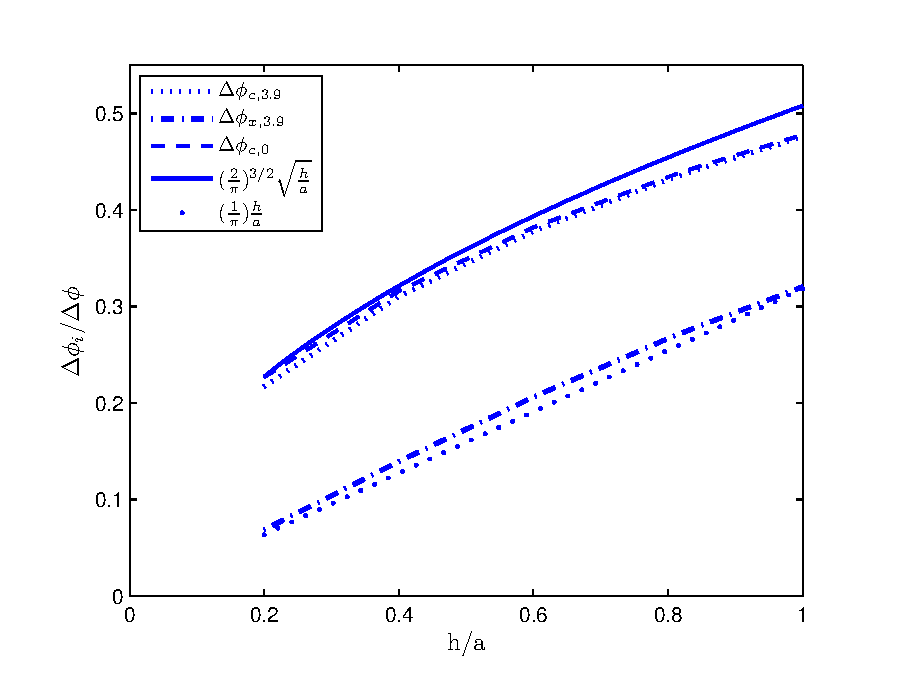
\includegraphics[width=0.8\textwidth,clip=true]{eddies/DeltaV_At_Corner_and_Axis2.eps}
\caption{The potential difference across the cylindrical pore, scaled by the
total potential difference $\Delta\phi$ between the two sides of the
membrane. Potential difference along the pore wall:
Solid line, theoretical prediction
$\Delta\phi_c$
(\ref{delta_phi_c});
dashed line, $\Delta\phi_{c,0}$ computed for $\epsilon_s=0$;
$\cdots$ 
computed for $\epsilon_s/\epsilon_0=3.9$.
Potential difference along the pore axis:
dotted line, $\Delta\phi_{c,3.9}$ 
theoretical prediction $\Delta\phi_x$ (\ref{delta_phi_x});
dash-dotted line, computed $\Delta\phi_{x,3.9}$ for $\epsilon_s/\epsilon_0=3.9$.
\label{fig:DeltaV}}
\end{figure}


\begin{figure}[ht]
\centering
\includegraphics[width=0.99\textwidth,clip=true]{eddies/eddy_fig4b.eps}
\caption{Numerically computed streamlines in the neighbourhood of the hole,
$a\kappa=5$, $\epsilon_s/\epsilon_0=3.9$. Uncharged membrane of thickness
(a) $h=0.4a$;
(b) $h=0.8a$;
(c) $h=0.84a$;
(d) $h=a$.
\label{fig:eddies}}
\end{figure}

The set of
time-independent equations governing the electrical potential
$\phi$, the ionic number densities $n^i$,
the fluid velocity $\mathbf{u}$ and fluid pressure $p$
consists of the Poisson equation (\ref{poisson}), the ion
conservation equation (\ref{ion_conservation}) and the Stokes equations
\begin{eqnarray}
-\nabla p + \mu \nabla^2 \mathbf{u} -  \nabla \phi \sum_{i=1}^{N} z_ien^i & = & 0, \label{eq:stokes_eddies}\\
\nabla \cdot \mathbf{u} & = & 0. \label{eq:continuity_eddies}
\end{eqnarray}
We solve the coupled equations (\ref{poisson}), (\ref{ion_conservation}),
(\ref{eq:stokes_eddies}),  and (\ref{eq:continuity_eddies})
by means of a finite volume numerical scheme based upon the
OpenFOAM CFD library \cite{OPENFOAM}.
The surface charge density $\sigma_\text{m}$ in the absence
of any imposed field
is set to zero, and a symmetrical electrolyte
($N=2$, $z_1=-z_2=1$)  is considered, with
identical cationic and anionic mobilities.
There is therefore complete symmetry about the plane of the
membrane, and no net flow through the hole. The relative permittivity
of the electrolyte
is $\epsilon_f/\epsilon_0=80$, where $\epsilon_0$ is the permittivity of
free space, and that of the membrane is set in the computations to be either
$\epsilon_\text{s}/\epsilon_0=3.9$,
corresponding to silica, or $\epsilon_s=0$.
The hole has radius $a=5\rm\ nm$ (a typical
hole size in silica \cite{Keyser2006} or graphene \cite{Garaj2010,Merchant2010}), with
$a\kappa=5$, corresponding to an electrolyte
of strength 95 mM (at 300 K).
The results presented here were performed with a mesh spacing
that varied smoothly from $\kappa^{-1}/10$
close to the membrane and hole, to $\kappa^{-1}$ at the far outer boundary.
The potential difference applied to generate the flow was $\Delta\phi=1\rm\ mV$,
so that $e\Delta\phi/kT\approx 0.04$: fluid velocities are
everywhere proportional
to $(\Delta\phi)^2$ as long as $e\Delta\phi/kT$ is sufficiently small
for the linearized Poisson-Boltzmann equation to be valid, in which case
the streamlines are independent of $\Delta\phi$.
Further details of the computational scheme are given by
Mao et al. \cite{mao2014}.

The difference in
electrical potential between the two ends of the
pore, at the wall of the cylindrical pore, is
$\Delta\phi_c$ (\ref{delta_phi_c}) when $h\ll a$
and this analytic prediction is shown
in Figure \ref{fig:DeltaV}
as a function of $h/a$. We see that the analytic result is in good 
agreement with computed results $\Delta\phi_{c,0}$ ($\epsilon_s=0$)
for $h/a<0.4$.
Also shown are computations for a membrane with relative permittivity
$\epsilon_s/\epsilon_0=3.9$, which differ little from those for
$\epsilon_s/\epsilon_0=0$.
If $h/a$ is sufficiently small, the resistance
of the pore changes only slightly \cite{sherwood2014} from that predicted for
the electric field (\ref{eq:chi_eddies})
when $h=0$.  We therefore expect the current along the
centreline of the pore, well away from the edges,
to be little changed, and the electric field
along the centreline is  still (to a first approximation)
$-\hat{\mathbf{z}}\Delta\phi/(a\pi)$
(\ref{Ez_hole}). The potential difference
between the ends ($z=\pm h/2$) of the pore along the centreline
should therefore be
\begin{equation}
\Delta\phi_x=\frac{\Delta\phi}{\pi}\left(\frac{h}{a}\right),\quad h\ll a.
\label{delta_phi_x}
\end{equation}
This too is shown in Figure \ref{fig:DeltaV}, and we see reasonable agreement
between theory and computation.

\begin{figure}[ht]
\centering
\includegraphics[width=0.99\textwidth,clip=true]{eddies/eddy_fig5.eps}
\caption{Schematic showing the boundaries of eddies in Figure \ref{fig:eddies}.
MA and GP represent the membrane surface at $z=h/2$; NC and EQ
the surface at $z=-h/2$. ABC and GFE represent the cylindrical surface of the
nanopore. Stagnation points within fluid (away from the walls)
are at (a) O,D,H, and (b) O,J,K. Axial symmetry implies that
the eddies ABD and GFH in (a) are cross-sections of the same toroidal eddy.
\label{fig:eddy_schematic}}
\end{figure}

When $\epsilon_s/\epsilon_0=3.9$, induced charges
lead to electro-osmosis.
Streamlines computed for the case $h=0.4a$ are shown in
Figure \ref{fig:eddies}(a) and take the form shown schematically in
Figure \ref{fig:eddy_schematic}(a).
Axial symmetry implies that ABD and GFH in Figure \ref{fig:eddy_schematic}(a)
are cross-sections of the same
toroidal eddy (and similarly for CBD and EFH).
However, the eddy pairs ABCD and EFGH in Figure \ref{fig:eddies}(a) are
very small. Flow near the corners A,C,E,G is a combination of the horizontal
velocity (\ref{u_thin_plane}) predicted on the upper and
lower surfaces of the membrane,
and the local corner flow (\ref{u_rho_wedge}), which flows upwards
along BA and FG, thereby causing the horizontal flow to separate at A and G
(and similarly at C and E).  At fixed position, the
uniform flow (\ref{u_thin_plane}) varies as $h^{-1}$, whereas the
corner flow (\ref{u_rho_wedge}) varies as 
$h^{-1/2}$. As $h$ increases, the ratio of the corner flow to horizontal flow
increases, and the eddies become larger, so that the stagnation
points D and H 
(or more correctly, stagnation lines, since the flow has axial symmetry)
move toward the central stagnation point at O.
This is seen in 
Figure \ref{fig:eddies}(b) for  $h=0.8a$.

When $h\approx 0.84a$ the stagnation points D and H merge into O, and
8 eddies meet at O, as seen in Figure \ref{fig:eddies}(c).
Any further increase in $h$ causes the
stagnation point to bifurcate into three points, at O, J and K, as
seen in Figure \ref{fig:eddies}(d) and shown schematically in
Figure \ref{fig:eddy_schematic}(b). Figure \ref{fig:eddies}(c)
shows eddies for $h=0.84a$, and the precise
value for $h$ at which the 8-fold stagnation point is formed lies
within the range $0.83a<h<0.85a$.
Computations with 
larger grid size $\kappa^{-1}/5$ in the vicinity of the membrane gave
streamlines that could not be distinguished from those in Figure
\ref{fig:eddies}, and the 8-fold stagnation point was still formed
at $h\approx 0.84a$,

The Debye length when $h=0.84a$ and $a\kappa=5$
is $\kappa^{-1}=0.238h$. The corner flow discussed in
Section \ref{sec:corner_charge} is valid only outside the charge
cloud (i.e. for $s>\kappa^{-1}$),
in which region the corner flow (\ref{u_s_corner})
is swamped by the velocity (\ref{u_thin_plane})
parallel to the plane of the membrane.
We are therefore unable 
to see in Figure \ref{fig:eddies} regions close to the corners
in which streamlines 
are symmetric about the local coordinate $\theta=0$ (Figure \ref{fig:corner}).

Any asymmetry in the flow caused by a non-zero
surface charge density $\sigma_\text{m}$
or by differences between the mobilities of the ions causes a net flow from
one side of the membrane to the other. If this is weak, the eddies
seen in Figure \ref{fig:eddies} persist, and the net flow has to snake its
way between them, as discussed by Jeffrey and Sherwood \cite{jeffrey1980},
Thamida and Chang \cite{Thamida2002}, and Yossifon {\it et al.}
\cite{yossifon2006}.


\section{Concluding remarks}

We have shown that the system of induced charge electro-osmotic eddies
in a cylindrical pore can have a rich structure that varies markedly
with pore aspect ratio. If flows created by induced charge electroosmosis
are strong
compared to net motion through the pore, there is a danger that
fluid trapped in the eddies may become contaminated (or may degrade)
over time, and lead to contamination of samples passing through the pore.
Such problems can be reduced by suitable choice of
pore geometry and imposed electric field strength, in order to control the
ratio of eddy velocity to volumetric flow rate through the pore.

We thank Professor E. Yariv (Technion) for helpful suggestions.
